\newpage
\chapter{Virtual Fixtures}

Virtual fixtures (VF), also called active constraints, are a family of algorithms used for limiting the workspace of the robot for safety and accuracy reasons, thus they are widely used in medical robotics. They were introduced in 1992~\cite{rosemberg1992use} by Rosemberg in an augmented reality teleoperation setup to simulate physical barriers, fields, and guides, designed to assist in the user during the teleoperation. 
VFs can be modelled with different shapes as shown in~\cite{bettini2004vision}where the author proposed a tube-like boundary with an admittance control and haptic feedback. Later on, different works show the crucial importance of VFs in medical robotics scenarios where the workspace of the robot must be limited to the area of interest to avoid hurting patients. In 2012 Rydén et al.~\cite{ryden2012forbidden} proposed an algorithm for the identification of a forbidden region virtual fixture from point clouds analysis that was used for operating on a beating hearth. The virtual fixture region is computed, considering each point of the point cloud as a 3D sphere with a particular radius. A known problem of VFs is the non passivity of the system when crossing or getting closer to the boundaries. 

\section{Classification of VFs}

A good classification of these algorithms is given in~\cite{bowyer2014active}. One of the most significant classifications is whether the fixture belongs to the \textit{forbidden region VF} or \textit{guidance VF}. The former bounds a manipulator’s tool to certain regions within its task or joint space, the latter encourages the user to move the tool along a specific pathway or toward a specific target. Usually, guidance constraints are more intrusive upon the user than forbidden region constraints in normal operation. The second meaningful classification for this work highlighted by the author is whether the constraint is \textit{unilateral} or \textit{bilateral}.
A unilateral virtual fixture is a constraint active only by one side, while the bilateral acts on both sides. 
Regional VFs (forbidden region) often are implemented with unilateral constraints, whereas guidance VFs leverage on bilateral limits.
The last distinction is between \textit{static} and \textit{dynamic} constraints that depend on if the geometry exploited by the algorithm change during the operation.

\section{VFs Generation}
In the literature, different methods for the generation of virtual fixture were proposed. The survey~\cite{bowyer2014active} mentions the most common types of constraint representations used in the literature.
\begin{enumerate}
    \item (a) Point: A single 3d point can be used to generate an attractive or repulsive potential field
    \item (b) Line: can be used to generate a guidance
    \item (c) Parametric curve: generalization of the line for task that requires some dexterity
    \item (d) Plane: Usually used as a forbidden region constraint to limit the robot workspace
    \item (e) Parametric surface: generalization of the plane. A well-known way for generating a parametric surface from a set of points is the Non Uniform Rational Basis-Splines (NURBS)
    \item (f) Polygonal Mesh: Non-parametric but realistic way of representing a real object. Can be used when the fidelity of the constraint is crucial for the task.
    \item (g) Point Cloud: A virtual fixture can be generated by a point cloud as explained in~\cite{ryden2012forbidden} 
    \item (h) Volumetric primitives: Boolean algebra can be applied to 3d mesh to obtain complex shapes maintaining computation efficiency in order to model situations in which the efficiency is critical
    \item (i) Explicitly described areas: work well in small scale scenarios but suffer from the curse of dimensionality.
\end{enumerate}
\begin{figure}[H]
    \centering   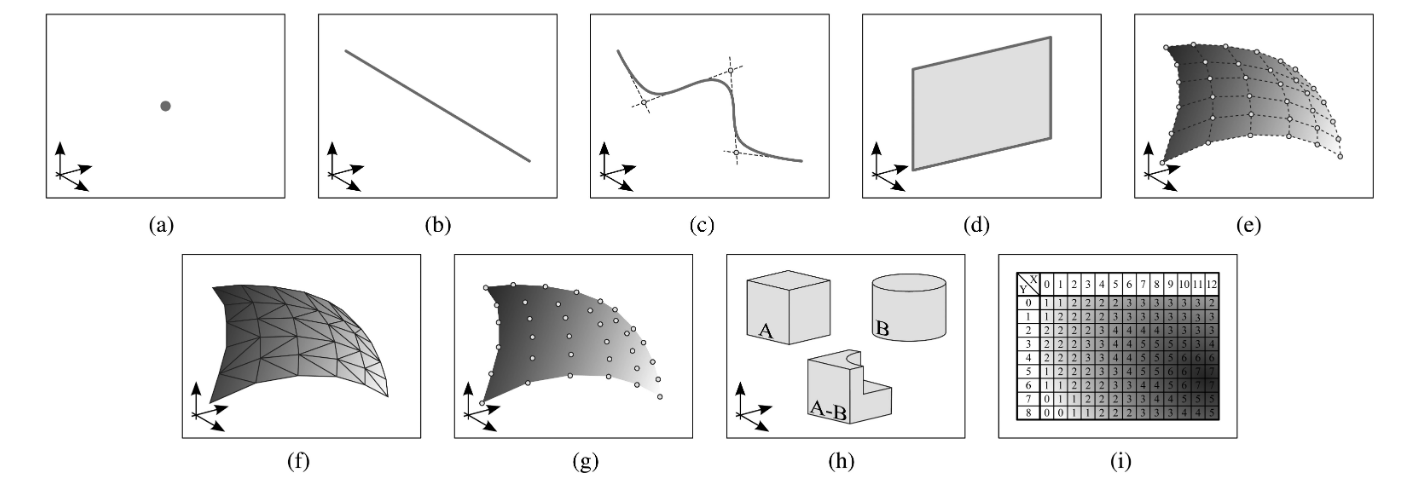
\includegraphics[width=0.7\linewidth]{images/virtual_fixtures/vf_geoms.png}
    \caption{The most common types of virtual fixture geometries reported by Bowyer et al.}
    \label{fig:virtual_fixture:vf_geoms}
\end{figure}
\TODO storia delle VF con reference
\cite{selvaggio2018passive}
\cite{soldati_proposal_2020}